\section{Discussion}
\label{sec:discussion}

\subsection{What the qualified two-registration evidence adds}

The central result is not that a lattice can approximate the Dirac equation.
That is known.  The intact evidence instead supports a shared core of one
bounded operational role across two sequentially tested, separately
prospective registered updates.  The product walk satisfies that core through
ordered local subdynamics; the direct QCA satisfies the same intact core
through a normalized symmetry-derived block with a different localization,
declared clock, and convergence signature, while its empirical zone-edge gate
is withdrawn.  The intact records support uniform propagator bounds, multiple
observables, and causal and symmetry constraints for both updates.
Algorithmically separate reconstruction agreed on those families while
duplicating the withdrawn $\pi$-sector predicate.  The result supports limited
robustness at the registered-specification level, not independence of the
underlying one-particle dynamics.

The coverage is only realization-level and enumerative: it covers these
two tested registered updates under the equivalence convention stated around
Eq.~\eqref{eq:time-frame-relation}.  The exact one-particle conjugacy rules out
any stronger claim that the two laws define algebraically independent
families.  ``Architecture independence'' would require a defined
architecture class and a theorem or sampling design over that class.  Nor do
the results support a primitive-class claim, because both constructions use
the same quantum substrate, periodic lattice, Born readout, and externally
specified clock and interventions.  The stronger value of the second
registration is therefore disciplined contrast, not unrestricted
generalization.

\subsection{Relation to established Dirac-QCA work}

Bisio, D'Ariano, and Tosini already derive the direct automaton, its exact
dispersion, low-mass/low-momentum Dirac regime, and a rigorous operational
comparison framed as channel discrimination
\citep{Bisio2015QuantumFieldQCA}.  They also establish Zitterbewegung and
potential scattering in the family \citep{Bisio2013DiracQCADynamics}.  Our
contribution does not supersede those results.  It embeds the established law
as the second side of a sequential two-registration study with a common role
core, realization-specific thresholds, an explicit direct-QCA full-space lift,
declared protocol clocks, precision accounting, single-use confirmation,
content-addressed ledgers, algorithmically separate reconstruction, and a
disclosed post-result defect audit.  The product full-space mass-mixer lift was
not comparably frozen.  That bounded package---not the generic idea of an
operational comparison, and not architecture-class breadth---is the novelty
claim.

\subsection{Global spectrum: a necessary boundary}

The direct QCA has exact principal band angle
\begin{equation}
 \omega(q,\mu)=\arccos\!\left(\sqrt{1-\mu^2}\cos q\right),
 \qquad q\in[-\pi,\pi).
 \label{eq:dispersion}
\end{equation}
For $0<|\mu|<1$, both the zero- and $\pi$-quasienergy circular gaps equal
$2\arcsin|\mu|$.  There is no additional zero-quasienergy cone in $1+1$
dimensions and hence no conventional low-energy doubler.  Independent
analysis of the one-dimensional Dirac quantum walk likewise finds no isolated
high-momentum/low-energy copy but does find a residual degeneracy under
simultaneous quasienergy and momentum shifts to Brillouin-zone corners,
motivating an explicit full-zone boundary even for a valid low-$q$ continuum
result \citep{Bakircioglu2025DoublingQCA}.  For
small zone-edge displacement $p$,
\begin{equation}
 U_\mu(-\pi+p)=-U_{-\mu}(p).
 \label{eq:pi-partner}
\end{equation}
After removal of the Floquet phase $-1$, the zone-edge mode has the same local
law with the opposite mass sign.  Following the distinction sharpened by
Gupta and Short \citep{Gupta2026FermionDoubling,Gupta2025DiracVacuum}, it is a
high-quasienergy pseudodoubler.  The registered low-$q$ result is not
invalidated: the input is separated from this sector, potential-generated
leakage is charged by the pre-outcome analytic bound, and the primary metric
compares propagators without asserting a global Hamiltonian logarithm.  The
intended empirical monitor is withdrawn under
Sec.~\ref{sec:post-result-audit}.  The identity
does, however, rule out a whole-zone or globally doubler-free interpretation.

At $\mu=0$, both circular gaps close and the principal logarithm becomes
branch-ambiguous at $q=-\pi$.  Accordingly, the effective-generator expansion
in Eq.~\eqref{eq:direct-effective} is confined to a branch-safe neighborhood of
$q=0$.  This reconciles a bounded continuum role with the global Floquet
spectrum and makes the limitation visible rather than relegating it to an
unmonitored high-momentum sector.

\begin{figure}[t]
  \centering
  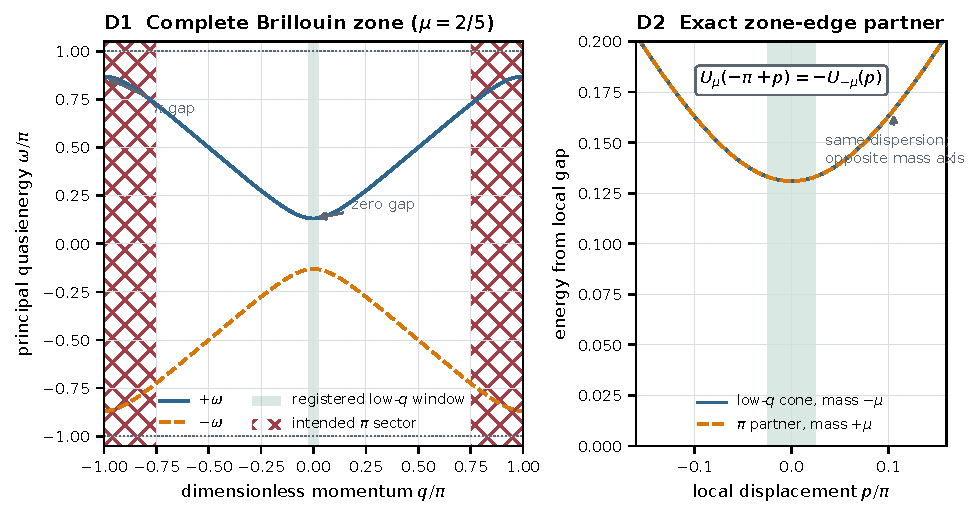
\includegraphics[width=\linewidth]{quantum_dirac_paper/figures/generated/fig04_spectrum_domain.pdf}
  \caption{\textbf{Global spectrum and bounded claim domain (\analytic; not a
  registered outcome).}  For the disclosed illustrative value $\mu=2/5$, the
  bands follow Eq.~\eqref{eq:dispersion}.  The central strip is the coarsest
  registered input window $|q|\le\pi/40$; finer windows are narrower.  Hatching
  marks the intended $\pi$ sector $|q|\ge3\pi/4$ used by the valid analytic
  tail; the empirical reducer for that sector is withdrawn.  The exact
  zone-edge identity exposes a high-quasienergy opposite-mass pseudodoubler.}
  \label{fig:spectrum}
\end{figure}

\subsection{Full-space lift and further tests}

The hard-core/fermionic collision-phase difference is not visible to any
one-excitation witness.  It becomes material under second quantization,
collisions, interactions, or a filled sea.  Published causal fermionic and
multiparticle QCA constructions show that those extensions require additional
structure \citep{Farrelly2014CausalFermions,Mlodinow2020QFTQCA}.  They cannot be
inferred from the present pass.  A canonical fermionic or interacting follow-on
should therefore receive a new search identifier, global-spectrum audit,
vacuum definition, and prospective protocol.

The direct hard-core lift is explicit, but the product registration does not
fix its mass mixer's vacuum and double-occupation phases.  The present
one-excitation comparison therefore supplies no product-versus-direct
collision claim.  A follow-on that uses full-space behavior must freeze both
lifts symmetrically.

The same separation applies to a differently localized circuit or a classical
reversible lattice gas.  A nominal Strang split is not automatically a third
case because Eq.~\eqref{eq:time-frame-relation} already exposes an exact
symmetric factorization of the direct block.  A genuinely new case would need
a predeclared circuit-equivalence criterion.  Either direction could increase
breadth, but neither
changes the interpretation of the completed two-registration result.  New
science should begin only after this manuscript's claims and limitations are
stable, under a separately registered search rather than as post-outcome
robustness tuning.

\begin{figure}[t]
  \centering
  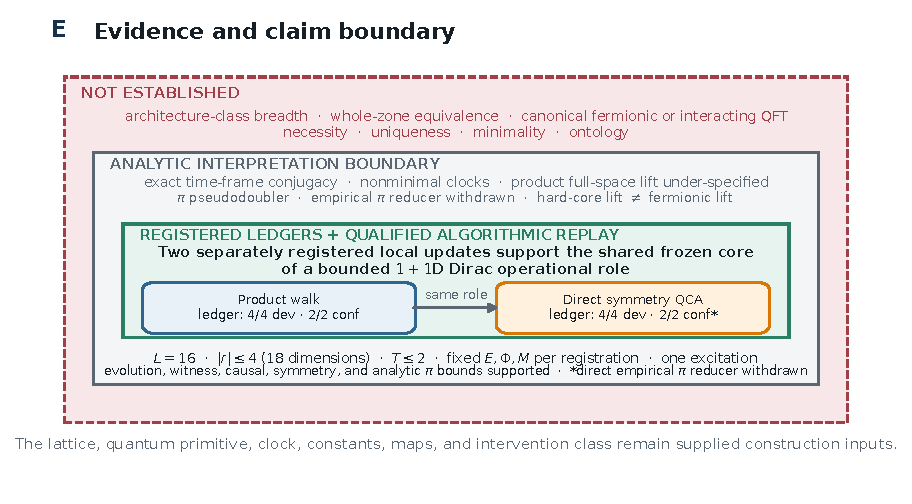
\includegraphics[width=\linewidth]{quantum_dirac_paper/figures/generated/fig05_claim_boundary.pdf}
  \caption{\textbf{Evidence and claim boundary (\conceptual{} synthesis).}
  The inner domain is the qualified registered result.  The middle domain contains
  analytic constraints required to interpret it.  The outer field lists
  claims not established.  Inclusion denotes logical scope, not evidential
  probability.  The withdrawn empirical $\pi$ reducer is shown as an audit
  boundary rather than positive evidence.}
  \label{fig:claim-boundary}
\end{figure}
